\subsection{Arrows}
\label{sec:arrows}
Arrows were introduced by \citet{HughesArrows} as a general interface for computation and a less restrictive generalisation of Monads. \citeauthor{HughesArrows} motivates the broader interface of Arrows with the example of a parser with added static meta-information that can not satisfy the monadic bind operator |(>>=) :: m a -> (a -> m b) -> m b| (with |m| being a Monad). In the example a parser of the type |Parser s a| with static meta information |s| and result |a| is shown to not be able to use the static information |s| without applying the monadic function |a -> m b|. With Arrows this is possible.

An Arrow |arr a b| represents a computation that converts an input |a| to an output |b|. This is defined in the |Arrow| type class shown in Fig.~\ref{fig:ArrowDefinition}.
%
To lift an ordinary function to an Arrow, |arr| is used, analogous to the monadic |return|. Similarly, the composition operator |>>>| is analogous to the monadic composition |>>=| and combines two arrows |arr a b| and |arr b c| by \enquote{wiring} the outputs of the first to the inputs to the second to get a new arrow |arr a c|. Lastly, the |first| operator takes the input Arrow |arr a b| and converts it into an arrow on pairs |arr (a, c) (b, c)| that leaves the second argument untouched. It allows us to to save input across arrows. Figure~\ref{fig:arrows-viz} shows a graphical representation of these basic Arrow combinators.
The most prominent instances of this interface are regular functions |(->)|
and the Kleisli type (Fig.~\ref{fig:ArrowDefinition}), which wraps monadic functions, e.g.  |a -> m b|.

\begin{figure}[t]
\centering
\begin{code}
class Arrow arr where
  arr :: (a -> b) -> arr a b
  (>>>) :: arr a b -> arr b c -> arr a c
  first :: arr a b -> arr (a,c) (b,c)

instance Arrow (->) where
	arr f = f
	f >>> g = g . f
	first f = \(a, c) -> (f a, c) 

data Kleisli m a b = Kleisli { run :: a -> m b }

instance Monad m => Arrow (Kleisli m) where
	arr f = Kleisli (return . f)
	f >>> g = Kleisli (\a -> f a >>= g)
	first f = Kleisli (\(a,c) -> f a >>= \b -> return (b,c))
\end{code}
\vfill
\caption{The definition of the |Arrow| type class and its two most typical instances.}
\label{fig:ArrowDefinition}
\end{figure}

\begin{figure}[t]
\centering
\parbox[c][17em]{0.49\linewidth}{%
\vfill
\centering
	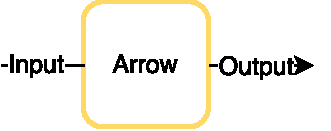
\includegraphics{images/arrow}
\vfill
%	\caption{Schematic depiction of an Arrow.}
%\label{fig:arrow-sch}
}
\parbox[c][17em]{0.49\linewidth}{%
\vfill
\centering
	{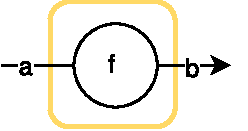
\includegraphics[scale=0.6]{images/arr}}
	{\includegraphics[scale=0.6]{images/compose}}
	{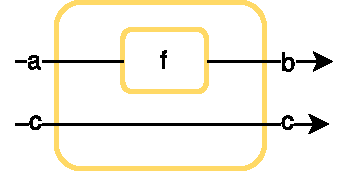
\includegraphics[scale=0.6]{images/first}}
\vfill
%\caption{Schematic depiction of |Arrow| combinators |arr|, |>>>| and |first|.}
%\label{fig:arrows-viz}
}
\caption{Schematic depiction of  an Arrow (left) and its basic
  combinators |arr|, |>>>| and |first| (right).}
\label{fig:arrow-sch}
\label{fig:arrows-viz}
\end{figure}

\begin{figure}[h]
	\centering
	\begin{tabular}{cc}
		% \subcaptionbox
{\label{t1}}{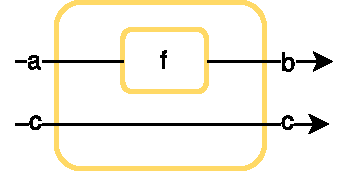
\includegraphics[width = 1.5in]{images/first}} &
		% \subcaptionbox
{\label{fig:secondImg}}{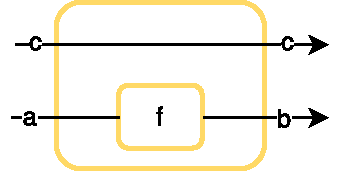
\includegraphics[width = 1.5in]{images/second}} \\
|first| & |second| \\
\midrule
		% \subcaptionbox
{}{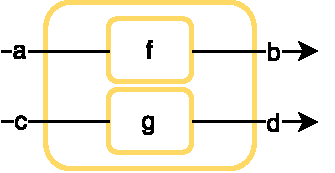
\includegraphics[width = 1.5in]{images/starstarstar}} &
		% \subcaptionbox
{}{\includegraphics[width = 1.5in]{images/andandand}}\\
|(***)|\label{fig:***Img} & |(&&&)| \label{fig:&&&Img} \\
	\end{tabular}
	\caption{Visual depiction of syntactic sugar for Arrows.}
	\label{fig:syntacticSugarArrows}
\end{figure}
Hughes also defined some syntactic sugar (Fig.~\ref{fig:syntacticSugarArrows}): |second|, |***| and |&&&|. 
|second| is the mirrored version of |first| (Appendix~\ref{utilfns}).
|***| combines |first| and |second| to handle two inputs in one arrow, and is defined as follows:
% \begin{figure}[h]
\begin{code}
(***) :: Arrow arr => arr a b -> arr c d -> arr (a, c) (b, d)
f *** g = first f >>> second g
\end{code}
% \caption{The (***) combinator}
% \label{fig:***}
% \end{figure}
The |&&&| combinator, which constructs an Arrow that outputs two different values like |***|, but takes only one input, is:
% \begin{figure}[h]
\begin{code}
(&&&) :: Arrow arr => arr a b -> arr a c -> arr a (b, c)
f &&& g = arr (\a -> (a, a)) >>> (f *** g)
\end{code}
% \caption{The (\&\&\&) combinator}
% \label{fig:&&&}
% \end{figure}
A~first short example given by Hughes on how to use arrows is addition with arrows:
%|add| over arrows, which can be seen in Fig.~\ref{fig:addArrows}.
% \begin{figure}[h]
\begin{code}
add :: Arrow arr => arr a Int -> arr a Int -> arr a Int
add f g = (f &&& g) >>> arr (\(u, v) -> u + v)
\end{code}

As we can rewrite the monadic bind operation |(>>=)| with only the Kleisli type into |m a -> Kleisli m a b -> m b|, but not with a general Arrow |arr a b|, we can intuitively get an idea of why Arrows must be a generalisation of Monads. While this also means that a general Arrow can not express everything a Monad can, the Parser example shows that this trade-off is worth it in some cases.

In this paper we will show that we can express parallel computations with Arrows and do not require Monads to do so. We also do not restrict the compatible Arrows to ones which have |ArrowApply| instances but instead only require instances for |ArrowChoice| and |ArrowLoop|. Because of this, we have a truly more general interface as compared to a monadic one.

Also note that, while we could have based our DSL on Profunctors as well, we chose Arrows. for this paper since they they are a more direct translation of pure functions than Profunctors. Note that Profunctors can easily be adapted to our interface as shown in Appendix~\ref{app:profunctorArrows}. However, they are a promising candidate for future improvements of our DSL.
